\documentclass{bookSolutions}

\title{Kreyszig  Introductory functional analysis with applications}
\author{Sergio Garrido}

\begin{document}
\maketitle

\tableofcontents

\section{Metric spaces}
\subsection{Metric space}

1 This is of course the most important metric space there is
2 Not so useful counterexample of a metric on R
4 There's infinitely many, but they're all kind of the "same"
5 Shows we can always multiply a metric with a number
6 Very important metric which ends up encoding uniform convergence 
8 Another very useful example of a metric leading eventually to the $L^1$ spaces 
9 The discrete metric is not so important except for counterexamples
11 Useful consequence of the triangle inequality
12 Useful consequence of the triangle inequality
13 Useful consequence of the triangle inequality
15 This one is pretty neat to see how some of the axioms are actually superfluous. Cool but not so important

\begin{exercise}{1}
Show that the real line is a metric space
\end{exercise}
\begin{proof}
fill
\end{proof}

\begin{exercise}{2}
Does $d(x,y)=(x-y)^2$ define a metric on the set of all real numbers?
\end{exercise}
\begin{proof}
fill
\end{proof}

\begin{exercise}{4}
Find all metrics on a set $X$ consisting of two points. Consisting of one point.
\end{exercise}
\begin{proof}
fill
\end{proof}

\begin{exercise}{5}
Let $d$ be a metric of $X$. Determine all constants $k$ such that (i) $kd$, (ii) $d+k$ is a metric on $X$
\end{exercise}
\begin{proof}
fill
\end{proof}

\begin{exercise}{6}
Show that $d$ in 1.1-6 satisfies the triangle inequality.
\end{exercise}
\begin{proof}
fill
\end{proof}

\begin{exercise}{8}
Show that another metric $\tilde{d}$ on the set $X$ in 1.1-7 is defined by $\tilde{d}(x,y)=\int_a^b\absoluteValue{x(t)-y(t)}dt$.
\end{exercise}
\begin{proof}
fill
\end{proof}

\begin{exercise}{9}
Show that $d$ in 1.1-8 is a metric.
\end{exercise}
\begin{proof}
fill
\end{proof}

\begin{exercise}{11}
Prove (1).
\end{exercise}
\begin{proof}
fill
\end{proof}

\begin{exercise}{12 (Triangle inequality)}
The triangle inequality has several useful consequences. For instance, using (1), show that $\absoluteValue{d(x,y)-d(z,w)}\leq d(x,z)+d(y,w)$
\end{exercise}
\begin{proof}
fill
\end{proof}

\begin{exercise}{13}
Using the triangle inequality show that $\absoluteValue{d(x,z)-d(y,z)}\leq d(x,y)$
\end{exercise}
\begin{proof}
fill
\end{proof}

\begin{exercise}{15}
Show that nonnegativity of a metric follows from (M2) to (M4).
\end{exercise}
\begin{proof}
fill
\end{proof}

\subsection{Further examples of metric spaces}


\begin{exercise}{3}
Show that the Cauchy-Schwarz inequality (11) implies 
\[
(\absoluteValue{x_1}+\dots+\absoluteValue{x_n})^2 
\leq n (\absoluteValue{x_1}^2+\dots+\absoluteValue{x_n}^2).
\]
\end{exercise}
\begin{proof}
Consider $(x_1,\dots,x_n)$ and $(1,\dots,1)$, $n$ times. Then the Cauchy-Schwarz inequality tells us
\[
\sum^n_{i=1}\absoluteValue{x_i} \leq
\sqrt{\sum_{i=1}^n\absoluteValue{x_i}^2}\sqrt{\sum_{i=1}^n\absoluteValue{1}^2} 
=\sqrt{\sum_{i=1}^n\absoluteValue{x_i}^2}\sqrt{n}.
\]
Squaring both sides of the inequality gives us the desired result.
\end{proof}

\begin{exercise}{4 (Space $l^p$)}
Find a sequence which converges to 0, but is not in any space $l^p$, where $1\leq p<+\infty$.
\end{exercise}
\begin{proof}
Consider the sequence $x_n=1/\log_2(n)$. This sequence converges to 0 because $\log_2(n)\to\infty$ as $n\to\infty$. However, we can do the Cauchy condensation test on the series $\sum_{n=1}^\infty 1/\absoluteValue{\log_2(n)}^p$ (to see whether $x_n$ is in $l^p$). We have 
\begin{align*}
    \sum_{n=1}^\infty \frac{2^n}{\absoluteValue{\log_2(2^n)}^p} 
    =\sum_{n=1}^\infty \frac{2^n}{\absoluteValue{n}^p}.
\end{align*}
Now using the ratio test on the sequence $2^n/\absoluteValue{n}^p$, we obtain
\[
\lim_{n\to\infty}\frac{2^{n+1}/\absoluteValue{(n+1)}^p}{2^n/\absoluteValue{n}^p} =2,
\]
so that the series does not converge for any $p$, giving us the desired result.
\end{proof}

\begin{exercise}{5}
Find a sequence which is in $l^p$ with $p>1$, but $x\notin l^1$.
\end{exercise}
\begin{proof}
We have that the series associated to the sequence $x_n=1/n$ does not converge for $p=1$ but it does for $p>1$, as required.
\end{proof}

\begin{exercise}{6 (Diameter, bounded set)}
The diameter $\delta(A)$ of a nonempty set $A$ in a metric space $(X,d)$ is defined to be 
\[
\delta(A) =\sup_{x,y\in A}d(x,y).
\]
$A$ is said to be bounded if $\delta(A)<\infty$. Show that $A\subseteq B$ implies $\delta(A)\leq\delta(B)$.
\end{exercise}
\begin{proof}
Since $\delta(B)=\sup{x,y\in B}d(x,y)$, then $\delta(B)$ is an upper bound for all the distances between the elements of $B$. However, because $A\subseteq B$, then the set of distances between the elements of $A$ is a subset of the set of distances between the elements of $B$. Hence $\delta(B)$ is also an upper bound for the set of distances between the elements of $A$. Thus, the least upper bound of such set, namely $\delta(A)$ is less than or equal to any other upper bound of such set, so that $\delta(A)\leq\delta(B)$, as required.
\end{proof}

\begin{exercise}{7}
Show that $\delta(A)=0$ (cf. exercise 6) if and only if $A$ consists of a single point.
\end{exercise}
\begin{proof}
Suppose $\delta(A)$ is 0, then for all $x,y\in A$, $d(x,y)=0$ (because $d$ is nonnegative), since $d(x,y)=0$ if and only if $x=y$, then $A$ consists of a single point. 

Conversely, suppose $A$ consists of a single point. Then $\delta(A) = \sup_{x,y\in A}d(x,y) =0$, as required.
\end{proof}

\begin{exercise}{11}
If $(X,d)$ is any metric space, show that another metric on $X$ is defined by
\[
\hat{d}(x,y)=\frac{d(x,y)}{1+d(x,y)},
\]
and $X$ is bounded in the metric $\hat{d}$.
\end{exercise}
\begin{proof}
M1, M2 and M3 follow directly from the properties of $d$ and the fact that the function $f(t)=t/(1+t)$ defined on the nonnegative reals does not alter these properties.

The proof that M4 holds for $\hat{d}$ is essentially the same as in 1.2-1, which I reproduce here for completeness. We have that $f'(t)=1/(1+t)^2$, which is positive, so that $f(t)$ is monotonically increasing. Thus, if $\absoluteValue{a+b}\leq \absoluteValue{a}+\absoluteValue{b}$, then $f(\absoluteValue{a+b})\leq f(\absoluteValue{a}+\absoluteValue{b})$. Knowing this, we have that 
\begin{align*}
    \frac{\absoluteValue{a+b}}{(1+\absoluteValue{a+b})} \leq& \frac{\absoluteValue{a}+\absoluteValue{b}}{1+\absoluteValue{a}+\absoluteValue{b}}\\
    \leq& \frac{\absoluteValue{a}}{1+\absoluteValue{a}} 
    + \frac{\absoluteValue{b}}{1++\absoluteValue{b}}.
\end{align*}
Replacing $a=d(x,z)$ and $b=d(z,y)$ in the above inequality we get the desired result.

To prove that $X$ is bounded under $\hat{d}$, consider the following two cases.

First: if $X$ is bounded under $d$, then $d(x,y)$ has an upper bound for all $x,y$ so that $\sup_{x,y\in X}\hat{d}(x,y)<\infty$.

Second: if $X$ is not bounded under $d$, then we have to check the limiting process of $\hat{d}$ whenever $d(x,y)\to\infty$ for some $x,y\in X$. In that case, we have $\lim_{d(x,y)\to\infty}\frac{d(x,y)}{1+d(x,y)}=1$, so that $\sup_{x,y\in X}\hat{d}(x,y)\leq \infty$, as required.
\end{proof}

\begin{exercise}{12}
Show that the union of two bounded sets $A$ and $B$ in a metric space is bounded. (Definition in exercise 6).
\end{exercise}
\begin{proof}
Suppose $A$ and $B$ are bounded. Let $a\in A\cup B$ be arbitrary and fix $a_0\in A$ and $b_0\in B$. If both $a_0,b_0$ are in either $A$ or $B$ then they they are bounded because both $A$ and $B$ are bounded. So suppose $a_0\in A$ and $b_0\in B$. By the generalised triangle inequality, with $x_1=a, x_2=a_0, x_3=b_0$ and $x_4=b$ (exercise 1.11), we obtain $d(a,b)\leq d(a,a_0)+d(a_0,b_0)+d(b_0,b)$. The first and the last terms of that inequality are bounded because $A$ and $B$ are bounded. Furthermore, by M1, $d(a_0,b_0)$ is finite. Thus, the right hand side of the inequality has an upper bound and since $a$ and $b$ were chosen arbitrarily, then $A\cup B$ is bounded.
\end{proof}

\begin{exercise}{13 (Product of metric spaces)}
The Cartesian product $X=X_1\times X_2$ of two metric spaces $(X_1, d_1)$ and $(X_2, d_2)$ can be made into a metric space $(X, d)$ in many ways. For instance, show that a metric $d$ is defined by $d(x,y)=d_1(x_1,y_1)+d_2(x_2,y_2)$, where $x=(x_1,x_2)$ and $y=(y_1,y_2)$.
\end{exercise}
\begin{proof}
M1, M2 and M3 follow from the fact that $d$ is an addition and the properties of $d_1$ and $d_2$. To see that M4 holds, let $x,y,z\in X_1\times X_2$. We have $d(x,y) =d_1(x_1,y_1)+d_2(x_2,y_2) \leq d_1(x_1,z_1)+d_1(z_1,y_1) + d_2(x_2,z_2)+d_2(z_2,y_2) = d(x,z)+d(z,y)$, as required.
\end{proof}

\begin{exercise}{14}
Show that another metric on $X_1\times X_2$ (as in exercise 13) is defined by $\hat{d}(x,y)=\sqrt{d_1(x_1,y_1)^2+d_2(x_2,y_2)^2}$.
\end{exercise}
\begin{proof}
M1, M2 and M3 follow directly from the properties of $d_1$ and $d_2$ and the functions that compose them: first squaring, then addition and then taking root, all of which preserve these properties of metrics. To see M4 holds, let $x,y,z\in X_1\times X_2$. We have 
\begin{align*}
    \hat{d}(x,y) =& [d_1(x_1,y_1)^2+d_2(x_2,y_2)^2]^{1/2}\\
    \leq& [[d_1(x_1,z_1)+d_1(z_1,y_1)]^2+[d_2(x_2,z_2)+d_2(z_2,y_2)]^2]^{1/2}\\
    =& [d_1(x_1,z_1)^2+2d_1(x_1,z_1)d_1(z_1,y_1)+d_1(z_1,y_1)^2\\
    &+ d_2(x_2,z_2)^2+2d_2(x_2,z_2)d_2(z_2,y_2)+d_2(z_2,y_2)^2]^{1/2}
\end{align*}
squaring both sides of the inequality, and using the the Cauchy-Schwarz inequality in those terms that contain a factor of 2:
\begin{align*}
    \hat{d}(x,y)^2 
    \leq&  d_1(x_1,z_1)^2+d_2(x_2,z_2)^2 +d_1(z_1,y_1)^2+d_2(z_2,y_2)^2\\
    &+2\sqrt{\sum_{i=1}^2d_i(x_i,z_i)^2}\sqrt{\sum_{i=1}^2d_i(z_i,y_i)^2}\\
    =& \hat{d}(x,z)^2 + \hat{d}(z,y)^2+ 2(\hat{d}(x,z)\hat{d}(z,y))\\
    =& (\hat{d}(x,z)+\hat{d}(z,y))^2.
\end{align*}
Taking square root on both sides of the inequality gives us the desired result.
\end{proof}

\begin{exercise}{15}
Show that a third metric on $X_1\times X_2$ (as in exercise 13) is defined by $\bar{d}(x,y)=\max[d_1(x_1,y_1),d_2(x_2,y_2)]$. (The metrics in exercises 13 to 15 are of practical importance, and other metrics on $X$ are possible).
\end{exercise}
\begin{proof}
M1, M2 and M3 follow directly from the properties of $d_1$ and $d_2$ and the fact that $\max$ does not affect these properties. To see M4 also holds, let $x,y,z\in X_1\times X_2$. We have
\begin{align*}
    \bar{d}(x,y) 
    =& \max[d_1(x_1,y_1),d_2(x_2,y_2)]\\
    \leq& \max[d_1(x_1,z_1)+d_1(z_1,y_1),d_2(x_2,z_2)+d_2(z_2,y_2)]\\
    \leq& \max[d_1(x_1,z_1),d_2(x_2,z_2)]
    + \max[d_1(z_1,y_1), d_2(z_2,y_2)]\\
    =& \bar{d}(x,z)+\bar{d}(z,y),
\end{align*}
where the last inequality follows from the fact that we are splitting the sums on the second line by choosing the greatest element of each sum and adding them together, hence the sum of the $\max$ is greater than the $\max$ of the sums.
\end{proof}
\section{Open set, closed set, neighborhood}


\begin{exercise}{1}
Justify the terms ``open ball'' and ``closed ball'' by proving that (a) any open ball is an open set, (b) any closed ball is a closed set.
\end{exercise}
\begin{proof}
(a) This follows the same logic as in the converse of exercise 4.

(b) Consider the closed ball with radius $r$ around $x$, $B=B(x;r)$. Let $y\in B^C$, and $r'=\min[d(y,x+r), d(y,x-r)]$, we have that $B(y;r'/2)\subseteq B^C$, so that for any point in $B^C$ there is an open ball containing it, that is, $B^C$ is open and thus $B$ is closed.
\end{proof}

\begin{exercise}{2}
What is an open ball $B(x_0; 1)$ on $\R$? In $\C$ (Cf. 1.1-5)?  In $C[a,b]$ (Cf. 1.1-7)? Explain the following figure.
\begin{figure}[H]
    \centering
    \includegraphics[width=0.5\textwidth]{kreyszig/assets/sec1-3-ex2.png}
    \caption{Region containing the graphs of all $x\in C[-1,1]$ which constitute the $\epsilon$-neighborhood, with $\epsilon=1/2$, of $x_0\in C[-1,1]$ given by $x_0(t)=t^2$.}
    \label{fig:fig1-3}
\end{figure}
\end{exercise}
\begin{proof}
$\R$: An open interval of the form $(a,b)$, where $b-a=2$ and the midpoint is $x_0$.

$\C$: If we think of $\C$ as $\R^2$ then it is a circle centered at $x_0$ with radius $1$, without the circumference of the circle.

$C[a,b]$: All the functions $g$ so that $\absoluteValue{g(t)-x_0(t)}<1$ for all $t$. 

We can see something similar in \Cref{fig:fig1-3}, where the shaded area is the area where the functions with $\absoluteValue{g(t)-t^2}<1/2$ can go through, for $t\in[-1,1]$.
\end{proof}

\begin{exercise}{3}
Consider $C[0,2\pi]$ and determine the smallest $r$ such that $g\in \hat{B}(f;r)$, where $f(t)=\sin t$ and $g(t)=\cos t$.
\end{exercise}
\begin{proof}
$r=1$ suffices, since the largest difference between $\sin t$ and $\cos t$ is 1 whenever $t=0$.
\end{proof}

\begin{exercise}{4}
Show that any nonempty set $A\subseteq (X,d)$ is open if and only if it is a union of open balls.
\end{exercise}
\begin{proof}
($\Rightarrow$) Suppose $A$ is open, then for every point in $x$ there is an open ball which is a subset of $A$. Thus $A$ is composed of open balls. That is, $A$ is a union of open balls.

($\Leftarrow$) Suppose $A$ is a union of open balls. Then any point in $x\in A$ belongs to one of these open balls, say $B(y;r)$. Let $r'=\min[d(x,y+r), d(x,y-r)]$, then $B(x;r')\subseteq B(y;r)\subseteq A$, so that there is an open ball around $x$ and $A$ is open.
\end{proof}

\begin{exercise}{5}
It is important to realise that certain sets may be open and closed at the same time. (a) Show that this is always the case for $X$ and $\emptyset$. (b) Show that in a discrete metric space $X$ (Cf. 1.1-8), every subset is open and closed.
\end{exercise}
\begin{proof}
(a) On page 19 Kreyszig proved that $\emptyset$ and $X$ are open. A set is closed if its complement is open. Hence given $X^C=\emptyset$ and $\emptyset^C=X$, both $X$ and $\emptyset$ are closed.

(b) From (a) we know that $X$ and $\emptyset$ are open and closed so let's consider a non trivial subset of $X$. Notice that every nonempty subset of $X$ is open, because for any $x\in X$, the set $\set{x}$ is a ball $B(x; r)$ for any $r<1$. But this means that the complement of any nonempty subset of $X$ is open because the same holds for any element of $X$. Hence, all subsets of $X$ are open and closed (clopen).
\end{proof}

\begin{exercise}{7}
Describe the closure of each of the following subsets. (a) The integers on $\R$, (b) the rational numbers on $\R$, (c) the complex numbers with rational real and imaginary parts in $\C$, (d) the disk $\set{z: \absoluteValue{z}<1}\subseteq\C$.
\end{exercise}
\begin{proof}
(a) Let $x\in\R$ and $x\notin\Z$. Notice that there are two integers $a,b$ so that $a<x<b$. Let $r=\min[x-a, b-x]$. We then have that $B(x,r)$ does not contain any element of $\Z$ and thus $x$ is not an accumulation point of $\Z$ in $\R$. As a result, $\Z=\overline{\Z}$ in $\R$.

(b) By the density of the rationals in the reals, any open ball around a rational contains an irrational number and hence it is an accumulation point. As a result, $\overline{\Q}=\R$.

(c) Following the same logic of (b), the closure of the complex numbers with rational real and imaginary parts is $\C$.

(d) This is similar to (b) and (c). Simply let $x\in\C$ have $\absoluteValue{x}=1$. For any $\epsilon>0$ we will always find that the ball $B(x;\epsilon)$ will contain an element of $\set{z: \absoluteValue{z}<1}$, so that $x\in\overline{\set{z: \absoluteValue{z}<1}}$. On the other hand, any number $y\in\C$ with $\absoluteValue{y}>1$ has an $\epsilon$-neighborhood so that no element of $\set{z: \absoluteValue{z}<1}$ belongs to it. Putting this together, we conclude that $\overline{\set{z: \absoluteValue{z}<1}}=\set{z: \absoluteValue{z}\leq 1}$.
\end{proof}

\begin{exercise}{8}
Show that the closure $\overline{B(x_0;r)}$ of an open ball $B(x_0;r)$ in a metric space can differ from the closed ball $\hat{B}(x_0;r)$.
\end{exercise}
\begin{proof}
Consider a set $X$ with the discrete metric. We have that $\hat{B}(x,1)=X$ for any $x\in X$. However, let $x,y\in X$ and consider the open ball $B(x;1)=\set{x}$. Think of the $\epsilon$-neighborhood around $y$ with $\epsilon=1/2$. Such $\epsilon$-neighborhood does not contain any element of $B(x;1)$, and so $y$ is not an accumulation point of $B(x;1)$. As a result, $B(x;1)=\overline{B(x;1)}\neq\hat{B}(x,1)=X$, as required.
\end{proof}

\begin{exercise}{9}
Show that 
\begin{enumerate}
    \item $A\subseteq\overline{A}$.
    \item $\overline{\overline{A}}=\overline{A}$.
    \item $\overline{A\cup B}=\overline{A}\cup\overline{B}$.
    \item $\overline{A\cap B}\subseteq\overline{A}\cap\overline{B}$.
\end{enumerate}
\end{exercise}
\begin{proof}
\begin{enumerate}
    \item By definition $\overline{A}$ contains $A$.
    \item We will prove this by double containment. $\overline{\overline{A}}\supseteq\overline{A}$ follows directly from the definition of closure. For the other direction, let $x\in \overline{\overline{A}}$. Then $x$ is either:
    
    (i) In $\overline{A}$, in which case $x\in\overline{\overline{A}}$ or,
    
    (ii) $x$ is an accumulation point of $\overline{A}$ not in $\overline{A}$.
    
    So suppose $x\notin \overline{A}$. Fix $\epsilon>0$, because $x$ is an accumulation point, there exists $y\in\overline{A}$ such that $d(x,y)\leq \epsilon/2$, and likewise because $y$ is in $A$ or it is one of its accumulation points, then  there exists $z\in A$ such that $d(y,z)\leq \epsilon/2$. Hence, $d(x,z)\leq d(x,y)+d(y,z) =\epsilon$ and so $x$ is an accumulation point of $A$ resulting in $x\in\overline{A}$. This contradicts (ii) so it must be the case that $x\in\overline{\overline{A}}$.
    \item We will prove this by double containment. 

    ($\subseteq$) Let $x\in\overline{A}\cup\overline{B}$. Then $x$ is either in $A$ or $B$ or an accumulation of either. If $x\in A$ or $x\in B$, then $x\in\overline{A}\cup\overline{B}$, so suppose $x\notin A,B$. Without loss of generality, suppose $x$ is an accumulation point of $A$. Then for every $\epsilon>0$, an open ball centered around $x$ with radius $\epsilon$ contains an element of $A$. But certainly it contains an element of $A\cup B$, so that $x\in\overline{A\cup B}$.

    ($\supseteq$) Let $x\in\overline{A\cup B}$. Then either $x\in A\cup B$ or $x$ is an accumulation of the union. In the former case, we would have that $x\in\overline{A}$ or $x\in\overline{B}$, so suppose that's not the case. Since $x$ is an accumulation point of $A\cup B$, then it must be the case there are infinite elements of $A\cup B$ that intersect open balls centered at $x$ (suppose this wasn't the case, then we could take the minimum of the distances between $x$ and every one of those elements of $A\cup B$, and then the open ball centered at $x$ with half such distance would not contain any element of $A\cup B$). However, this implies that there are either infinite elements of $A$ or infinite elements of $B$ that intersect open balls centered around $x$ (of any arbitrarily small radius), so that either $x\in\overline{A}$ or $x\in\overline{B}$.
    \item Suppose $x\in\overline{A\cap B}$, then either $x\in A\cap B$ or $x$ is an accumulation point of such set. If $x\in A\cap B$, then $x\in A$ and $x\in B$ so certainly $x\in\overline{A}\cap\overline{B}$ since $A\subseteq\overline{A}$ and $B\subseteq\overline{B}$. So suppose $x$ is an accumulation point of $A\cap B$. This implies that for every $\epsilon>0$, the open ball of radius $\epsilon$ centered at $x$ contains an element $y\in A\cap B$. Thus, for every $\epsilon>0$, there exists an element of $A$ such that it belongs to the open ball centered around $x$, so that $x\in\overline{A}$, following the same argument we can conclude that $x\in\overline{B}$ as well. That is, $x\in\overline{A}\cap\overline{B}$.
    \end{enumerate}
\end{proof}

\begin{exercise}{11 (Boundary)}
A boundary point $x$ of a set $A\subseteq (X,d)$ is a point of $X$ (which may or may not belong to $A$) such that every neighborhood of $x$ contains points of $A$ as well as points not belonging to $A$; and the boundary (or frontier) of $A$ is the set of all boundary points of $A$. Describe the boundary of (a) the intervals $(-1,1), [-1,1), [-1,1]$ on $\R$; (b) the set of all rational numbers on $\R$; (c) the disks $\set{z:\absoluteValue{z}<1}\subseteq\C$ and $\set{z:\absoluteValue{z}\leq 1}\subseteq\C$.
\end{exercise}
\begin{proof}
(a) For all intervals $-1$ and 1 are the boundary points. Simply consider for any $\epsilon>0$ the open ball around any of these two points. We will obtain than points in the intervals (and outside of them), are in such ball.

(b) Since the rationals are dense in $\R$, any open ball around any rational will contain both rationals and irrationals. Furthermore, for any irrational, we can find a rational that gets arbitrarily close to it. Hence, $\R$ is the boundary of $\R$.

(c) In both cases, the set $\set{z:\absoluteValue{z}=1}\subseteq\C$ is the boundary of the disks. That is because for any open ball around these points, we can find elements withing the disks and outside of them.
\end{proof}

\begin{exercise}{12 (Space $B[a,b]$)}
 Show that $B[a,b]$, $a<b$ is not separable (Cf. 1.2-2).
\end{exercise}
\begin{proof}
Suppose, for the sake of contradiction, that $B[a,b]$ is separable. Then there exists a countable set, call it $\cF$, of functions so that for all functions in $g\in B[a,b]$, either $g\in\cF$, or for all $\epsilon>0$, there exists a function $f\in\cF$ with $f\in B(g;\epsilon)$.

Since $\cF$ is countable we can find a bijection between $\cF$ and $\N$, so that we can have a sequence of distinct numbers, $(x_n)$ where each $x_i\in[a,b]$ and $x_n$ can be mapped to a function, say $f_n\in\cF$. Now let $h\in B[a,b]$ be defined as follows: for $h(x_n)=f_n(x_n)+1$ and 0 otherwise. We have that the open ball $B(h;1/2)$ does not contain any element of $\cF$, so that $h$ is not an accumulation point of $\cF$. Thus, $\overline{\cF}\neq B[a,b]$ and $B[a,b]$ is not separable. 
\end{proof}

\begin{exercise}{13}
Show that a metric space $X$ is separable if and only if $X$ has a countable subset $Y$ with the following property. For every $\epsilon>0$ and every $x\in X$ there is a $y\in Y$ such that $d(x,y)<\epsilon$.
\end{exercise}
\begin{proof}
($\Rightarrow$) Suppose $X$ is separable. Then there exists a countable subset $Y\subseteq X$ so that $\overline{Y}=X$. But this means that for every $x\in X$, either $x\in Y$ or that for all $\epsilon>0$, there exists a $y\in Y$ with $y\in B(x, \epsilon)=\set{z\in X:d(x,z)<\epsilon}$, giving us the desired result.

($\Leftarrow$) Suppose there exists a countable subset $Y\subseteq X$ so that for every $\epsilon>0$, and every $x\in X$, there exists a $y\in Y$ with $d(x,y)<\epsilon$. Then this means that every $x\in X$ is an accumulation point, because for every $x$ and $\epsilon>0$ we can find $y\in Y$ with $y\in B(x,\epsilon)$. However, since all $x\in X$ are accumulation points of $Y$, then $\overline{Y}=X$, giving us that $X$ is separable, as required.
\end{proof}

\begin{exercise}{14 (Continuous mapping)} Show that a mapping $T:X\to Y$ is continuous if and only if the inverse image of any closed set $M\subseteq Y$ is a closed set in $X$.
\end{exercise}
\begin{proof}
Let $M$ be closed so that $M^C$ is open. By definition, we have that $(T^{-1}(M))^C=\set{x\in X:T(x)\notin M}=T^{-1}(M^C)$. 

For the ($\Rightarrow$) proof, if $T$ is continuous, then the inverse image of an open set is open, so that $T^{-1}(M^C)$ is open and by the equality above, then the inverse image of a closed set is closed. That is, $(T^{-1}(M))^C$ is open. 

For the converse, $(\Leftarrow)$, if the inverse image of a closed set is closed, so that $(T^{-1}(M))^C$ is open, by the equality above, we get that $T^{-1}(M^C)$ is open, so that the inverse image of an open set is open. That is, $T$ is continuous.
\end{proof}

\begin{exercise}{15}
Show that the image of an open set under a continuous mapping need not be open.
\end{exercise}
\begin{proof}
We have that $f:\R\to\R$ given by $f(x)=x^2$ is continuous. Consider the open set $A=(-1,1)\in\R$. We have that $f(A)=[0,1)$, which is not open in $\R$ because there is no open ball around 0 fully contained in $[0,1)$.
\end{proof}

\subsection{Convergence, Cauchy sequence, completeness}

2
3
4
5
6 Basic facts about convergence
8
9 We call these metrics to be equivalent. Equivalent metrics are not the same but enjoy mostly the same properties when it comes to sequence convergence, Cauchy, completeness, etc.
10

\begin{exercise}{1 (Subsequence)}
If a sequence $(x_n)$ in a metric space $X$ is convergent and has limit $x$, show that every subsequence $(x_{n_k})$ of $(x_n)$ is convergent and has the same limit $x$.
\end{exercise}
\begin{proof}
Let $(x_{n_k})$ be a subsequence of $(x_n)$. Since $(x_n)$ converges to $x$, then for all $\epsilon>0$, there exists an $N\in\N$ so that for all $n>N$, it holds that $d(x_n,x)<\epsilon$. Fix $\epsilon>0$, and find $N\in\N$ as above. Now $N=n_K$ for some $K\in\N$, so that for all $k>K$ (and thus $n_k>N$, it holds that $d(x_{n_k},x)<\epsilon$ and $(x_{n_k})\to x$, as desired.
\end{proof}

\begin{exercise}{2}
If $(x_n)$ is Cauchy and has a convergent subsequence, say, $x_{n_k}\to x$, show that $(x_n)$ is convergent with the limit $x$.
\end{exercise}
\begin{proof}
fill
\end{proof}

\begin{exercise}{3}
Show that $x_n\to x$ if and only if for every neighborhood $V$ of $x$ there is an integer $n_0$ such that $x_n\in V$ for all $n>n_0$.
\end{exercise}
\begin{proof}
fill
\end{proof}

\begin{exercise}{4 (Boundedness)}
Show that a Cauchy sequence is bounded.
\end{exercise}
\begin{proof}
fill
\end{proof}

\begin{exercise}{5}
Is boundedness of a sequence in a metric space sufficient for the sequence to be Cauchy? Convergent?
\end{exercise}
\begin{proof}
fill
\end{proof}

\begin{exercise}{6}
If $(x_n)$ and $(y_n)$ are Cauchy sequences in a metric space $(X,d)$, show that $(a_n)$, where $a_n=d(x_n,y_n)$, converges. Give illustrative examples.
\end{exercise}
\begin{proof}
fill
\end{proof}

\begin{exercise}{8}
If $d_1$ and $d_2$ are metrics on the same set $X$ and there are positive numbers $a$ and $b$ such that for all $x,y\in X$, $ad_1(x,y)\leq d_2(x,y)\leq bd_1(x,y)$, show that the Cauchy sequences in $(X,d_1)$ and $(X,d_2)$ are the same.
\end{exercise}
\begin{proof}
fill
\end{proof}

\begin{exercise}{9}
Using exercise 9, show that the metric space in exercises 13 to 15 of Section 1.2 have the same Cauchy sequences.
\end{exercise}
\begin{proof}
fill
\end{proof}

\begin{exercise}{10}
Using the completeness of $\R$, prove the completeness of $\C$.
\end{exercise}
\begin{proof}
fill
\end{proof}
\subsection{Examples. Completeness proofs}

1 Can you find an easy criterion which subsets of R are complete?
2 $R^n$ is complete with different metrics, including this one, which is occasionally useful
3 Example of a noncomplete infinite dimensional space 
5 Example of a completeness proof
6 This is a pretty cool example since with this metric we can treat limits to infinity or being infinity on the same level as usual limits
8 Infinite dimensional completeness proof 
10 Example of a completeness proof
11
12 We see here that the space s has convergence the same as pointwise convergence, in the same way convergence in $l^infinity$ and C[a,b] is uniform convergence. The space s won't really occur too much in Kreyszig however, but it would in Carothers and general topo

\begin{exercise}{1}
Let $a,b\in\R$ and $a<b$. Show that the open interval $(a,b)$ is an incomplete subspace of $\R$, whereas the closed interval $[a,b]$ is complete.
\end{exercise}
\begin{proof}
fill
\end{proof}

\begin{exercise}{2}
Let $X$ be the space of all ordered $n$-tuples $x=(x_1,x_2,\dots,x_n)$ of real numbers and $d(x,y)=\max_j\absoluteValue{x_j,y_j}$ where $y=(y_n)$. Show that $(X,d)$ is complete.
\end{exercise}
\begin{proof}
fill
\end{proof}

\begin{exercise}{3}
Let $M\subseteq l^\infty$ be the subspace consisting of all sequences $x=(x_n)$ with at most finitely many nonzero terms. Find a Cauchy sequence in $M$ which does not converge in $M$, so that $M$ is not complete.
\end{exercise}
\begin{proof}
fill
\end{proof}

\begin{exercise}{5}
Show that the set $X$ of all integers with metric $d$ defined by $d(m,n)=\absoluteValue{m-n}$ is a complete metric space.
\end{exercise}
\begin{proof}
fill
\end{proof}

\begin{exercise}{6}
Show that the set of all real numbers constitutes an incomplete metric space if we choose $d(x,y)=\absoluteValue{\arctan x-\arctan y}$.
\end{exercise}
\begin{proof}
fill
\end{proof}

\begin{exercise}{8 (Space $C[a,b]$)}
Show that the subspace $Y\subseteq C[a,b]$ consisting of all $x\in C[a,b]$ such that $x(a)=x(b)$ is complete
\end{exercise}
\begin{proof}
fill
\end{proof}

\begin{exercise}{10 (Discrete metric)}
Show that a discrete metric space (cf. 1.1-8) is complete.
\end{exercise}
\begin{proof}
fill
\end{proof}

\begin{exercise}{11 (Space $s$)}
Show that in the space $s$ (cf. 1.2-1) we have $x_n\to x$ if and only if $x^n_j\to x_j$ for all $j=1,2,\dots$, where $x_n=(x^n_j)$ and $x=(x_j)$.
\end{exercise}
\begin{proof}
fill
\end{proof}

\begin{exercise}{12}
Using exercise 11, show that the sequence space $s$ in 1.2-1 is complete.
\end{exercise}
\begin{proof}
fill
\end{proof}
\section{Completion of metric spaces}


\begin{exercise}{1}
Show that if a subspace $Y$ of a metric space consists of finitely many points, then $Y$ is complete.
\end{exercise}
\begin{proof}
To prove $Y$ is complete we will use Theorem 1.4-7. We will prove $Y$ is closed by proving $Y^C$ is open. Let $r=\min_{x,y\in Y}d(x,y)$. Then for all $x\in Y^C$, the ball $B(x;r)\subset Y^C$, because there is no point in $Y$ with distance less than $r$ to $x$. Thus $Y^C$ is open, $Y$ is closed, and by Theorem 1.4-7, $Y$ is complete.
\end{proof}

\begin{exercise}{2}
What is the completion of $(X,d)$, where $X$ is the set of all rational numbers and $d(x,y)=\absoluteValue{x-y}$.
\end{exercise}
\begin{proof}
The reals, as we can get arbitrarily close to any real number using rational numbers and the reals are complete.
\end{proof}

\begin{exercise}{3}
What is the completion of a discrete metric space $X$? (Cf.1.1-8).
\end{exercise}
\begin{proof}
In exercise 1.5.10 we proved discrete metric spaces are complete, thus, their completions are themselves.
\end{proof}

\begin{exercise}{4}
If $X_1$ and $X_2$ are isometric and $X_1$ is complete, show that $X_2$ is complete.
\end{exercise}
\begin{proof}
We have that $\overline{X_1}=X_1$, that is, $X_1$ equals its completion. By Theorem 1.6-2, $\overline{X_1}$ is unique up to isometries. Since $X_2$ is isometric to $X_2$, then it must be the case that $X_2$ is complete, since $X_1$ is complete too.
\end{proof}

\begin{exercise}{5 (Homeomorphism)}
A homeomorphism is a continuous bijective mapping $T:X\to Y$ whose inverse is continuous; the metric spaces $X$ and $Y$ are then said to be homeomorphic. (a) Show that if $X$ and $Y$ are isometric, they are homeomorphic. (b) Illustrate with an example that a complete and an incomplete metric space may be homeomorphic.
\end{exercise}
\begin{proof}
a) If $X$ and $Y$ are isometric, then there exists a bijective function $T:X\to Y$ so that $\bar{d}(Tx,Ty)=d(x,y)$ for all $x,y\in X$. Hence, to prove that $X$ and $Y$ are homeomorphic, we need to prove that $T$ and $T^{-1}$ are both continuous. 

Fix $\epsilon>0$, we have $\bar{d}(Tx,Ty)=d(x,y)<\epsilon$ so that by choosing $\delta=\epsilon$ we can make $Tx$ and $Ty$ arbitrarily close. Since $T$ is bijective and continuous, then its inverse is also continuous. Hence, $X$ and $Y$ are homeomorphic.

b) The metric space $(X,d)$ with $X=(-\pi/2,\pi/2)$ and $d$ being the usual metric in $\R$. These spaces are homeomorphic with $f:X\to\R$ defined by $f(x)=\tan x$ being bijective and continuous for all $x\in X$. However, $X$ is not complete, given that $\pi/2$ is a limit point (that is, it is the limit of a Cauchy sequence in $X$) of $X$ but not in $X$.
\end{proof}

\begin{exercise}{9}
If $(x^n)$ and $(y^n)$ in $(X,d)$ are such that (1) holds and $(x^n)\to x$, show that $(y^n)$ converges and has the limit $x$.
\end{exercise}
\begin{proof}
Suppose $\lim_{n\to\infty}d(x^n,y^n)=0$ so that there exists $N\in\N$ with $d(x^n,y^n)<\epsilon/2$ for $n>N$. Furthermore, we assume $(x^n)\to x$, so that for $\epsilon>0$, there exists an $N'\in\N$ with $d(x^n,x)<\epsilon/2$ for $n>N'$. 

Let $M=\max[N,N']$ and $n>M$. We have $d(y^n, x)\leq d(y^n,x^n)+d(x^n,x)<\epsilon$, so that $(y^n)\to x$, as required.
\end{proof}

\begin{exercise}{10}
If $(x^n)$ and $(y^n)$ are convergent sequences in a metric space $(X,d)$ and have the same limit $x$, show that they satisfy $\lim_{n\to\infty}d(x^n,y^n)=0$.
\end{exercise}
\begin{proof}
Since $(x^n)\to x$ and $(y^n)\to x$, then for $\epsilon>0$, there exist $N,N'\in\N$ so that for $n>N$ and $m>N'$, we have both $d(x^n,x)<\epsilon/2$ and $d(y^m,x)<\epsilon/2$. Thus, let $n>\max[N,N']$, consider $d(x^n,y^n)\leq d(x^n,x)+d(x,y^n)<\epsilon$, giving us $\lim_{n\to\infty}d(x^n,y^n)=0$, as required.
\end{proof}

\begin{exercise}{11}
Show that (1) defines an equivalence relation on the set of all Cauchy sequences of elements of $X$.
\end{exercise}
\begin{proof}
Let $(x^n), (y^n)$ and $(z^n)$ be Cauchy in $X$.

Reflexivity: We have $d(x^n,x^n)=0$ for all $n$, so that $\lim_{n\to\infty}d(x^n,x^n)=0$.

Symmetry: We have $d(x^n,y^n)=d(y^n,x^n)$, for all $n$, so that $\lim_{n\to\infty}d(x^n,y^n)=\lim_{n\to\infty}d(y^n,x^n)$.

Transitivity: If $\lim_{n\to\infty}d(x^n,y^n)=0$ and $\lim_{n\to\infty}d(y^n,z^n)=0$. We have $d(x^n,z^n)\leq d(x^n,y^n)+d(y^n,z^n)$. Taking limits on both sides gives us that $\lim_{n\to\infty}d(x^n,z^n)=0$.
\end{proof}

\begin{exercise}{12}
If $(x^n)$ is Cauchy in $(X,d)$ and $(y^n)$ in $X$ satisfies $\lim_{n\to\infty}d(x^n,y^n)=0$, show that $(y^n)$ is Cauchy in $X$.
\end{exercise}
\begin{proof}
Suppose $(x^n)$ is Cauchy and $\lim_{n\to\infty}d(x^n,y^n)=0$. Fix $\epsilon>0$. There exists $N\in\N$ so that for all $n,m>N$, it holds that $d(x^n,x^m)<\epsilon/3$. Moreover, there exists $N'\in\N$ so that $d(x^n,y^n)<\epsilon/3$. We have $d(y^n,y^m)\leq d(y^n,x^n)+d(x^n,y^m)\leq d(y^n,x^n)+d(x^n,x^m)+d(x^m,y^m)<\epsilon$, so that $(y^n)$ is Cauchy as required.
\end{proof}

\begin{exercise}{13 (Pseudometric)}
A finite pseudometric on a set $X$ is a function $d:X\times X\to\R$ satisfying (M1), (M3), (M4), section 1.1, and 
\[
\text{(M2)}^\ast\quad d(x,x)=0.
\]
What is the difference between a metric and a pseudometric? Show that $d(x,y)=\absoluteValue{x_1-y_1}$ defines a pseudometric on the set of all ordered pairs of real numbers, where $x=(x_1,x_2)$, $y=(y_1,y_2)$. (We mention that some authors use the term semimetric instead of pseudometric).
\end{exercise}
\begin{proof}
The difference between a metric and pseudometric is that a pseudometric can have 0 distance between non distinct points. That is, it is not the case that $d(x,y)=0$ if and only if $x=y$.

(M1): Certainly $d$ is real valued, finite and nonnegative. 

$\text{(M2)}^\ast$: For any $x\in X$, $d(x,x)=0$.

(M3): For any $x,y\in X$, we have $d(x,y)=\absoluteValue{x_1-y_1}=\absoluteValue{y_1-x_1}=d(y,x)$.

(M4): For $x,y,z\in X$ we have $d(x,y)=\absoluteValue{x_1-y_1}\leq \absoluteValue{x_1-y_1}+\absoluteValue{y_1-z_1}=d(x,y)+d(y,z)$.

Remark: Consider the pairs $x=(1,1)$ and $y=(1,0)$. We have that $d(x,y)=0$, however, $x\neq y$.
\end{proof}

\begin{exercise}{14}
Does 
\[
d(f,g)=\int^b_a\absoluteValue{f(t)-g(t)}dt
\]
define a metric or pseudometric on $X$ if $X$ is (a) the set of all real-valued continuous functions on $[a,b]$, (b) the set of all real-valued Riemann integrable functions on $[a,b]$?
\end{exercise}
\begin{proof}
Without loss of generality, let $a=0$ and $b=1$.
a) We will prove that $d$ is a metric on the set of continuous functions. If $f=g$, then for $h=f-g$ we have $\int^1_0\absoluteValue{h(x)}dx=0$. Now suppose $f\neq g$. Since both $f$ and $g$ are continuous, then $h$ is continuous, and moreover, there is a point at which $\absoluteValue{h}$ is nonzero. Because $h$ is continuous, then there must be a neighborhood around that point which is positive, so that $\int^1_0\absoluteValue{h(x)}dx> 0$, as required.

b) Let $f(x)=0$ for $x\in(0,1]$ and $f(0)=1$; $g(x)=0$ for $x\in[0,1)$ and $g(1)=1$. We have that both $f$ and $g$ are Riemann integrable and that $\absoluteValue{f-g}(x)=0$ for $x\in(0,1)$ and 1 otherwise. Moreover, $d(f,g)=0$, so that $d$ is a pseudometric on the set of all real-valued Riemann integrable functions.
\end{proof}


\section{Normed spaces. Banach spaces}
\subsection{Vector space}

\begin{exercise}{1}
fill
\end{exercise}
\begin{proof}
fill
\end{proof}
\subsection{Normed space. Banach space}

\begin{exercise}{1}
fill
\end{exercise}
\begin{proof}
fill
\end{proof}
\subsection{Further properties of normed spaces}

\begin{exercise}{1}
fill
\end{exercise}
\begin{proof}
fill
\end{proof}
\subsection{Finite dimensional normed spaces and subspaces}

\begin{exercise}{1}
fill
\end{exercise}
\begin{proof}
fill
\end{proof}
\subsection{Compactness and finite dimension}

\begin{exercise}{1}
fill
\end{exercise}
\begin{proof}
fill
\end{proof}
\subsection{Linear operators}

\begin{exercise}{1}
fill
\end{exercise}
\begin{proof}
fill
\end{proof}
\subsection{Bounded and continuous linear operators}


\begin{exercise}{1}
Let $X,Y,Z$ be normed spaces, and $T_1:Y\to Z$ and $T_2:Y\to Z$ and $T:X\to X$ bounded linear operators. Then:
\begin{enumerate}
    \item $\norm{T_1T_2}\leq\norm{T_1}\norm{T_2}$, and
    \item $\norm{T^n}\leq \norm{T}^n$, for all $n\in\N$.
\end{enumerate}
\end{exercise}
\begin{proof}
Notice that for all $x\in\DDD(T_1,T_2)$ we have
\[
\norm{T_1T_2x}\leq\norm{T_1}\norm{T_2x}\leq\norm{T_1}\norm{T_2}\norm{x},
\]
so that dividing both sides of the inequality by $\norm{x}$ we get that $\norm{T_1T_2}\leq\norm{T_1}\norm{T_2}$, as required.

The second inequality follows from induction, by using $T=T_1=T_2$ in the first step, and $T=T_1$ and $T^{n-1}=T_2$ on the induction step.
\end{proof}

\begin{exercise}{2}
Let $X$ and $Y$ be normed spaces. 
Show that a linear operator $T:X\to Y$ is bounded if and only if $T$ maps bounded sets in $X$ into bounded sets in $Y$.
\end{exercise}
\begin{proof}
($\Rightarrow$) Let $T$ be bounded. Then there exists a constant $c$ so that for all $x\in X$, we have $\norm{Tx}\leq c\norm{x}$. Let $A\subseteq X$ be bounded. Hence, $\sup_{x,y\in A}\norm{x-y}=M<\infty$. Thus, $\norm{T(x-y)}=\norm{Tx-Ty}\leq c\norm{x-y}<\infty$ so that the set $T(A)$ is bounded too.

($\Leftarrow$) Let $T$ map bounded sets to bounded sets, so that if $A\subseteq X$ is a bounded set, then $T(A)\subseteq Y$ is bounded too. Let $A=\set{x\in X:\norm{x}=1}$. To see this is a bounded set, notice that if $x,y\in A$, then $d(x,y)\leq d(x,0)+d(0,y) =\norm{x}+\norm{y}=2$. By exercise 2.2.15, we have that $A$ is bounded if and only if there is a positive number $c$ such that $\norm{x}\leq c$ for all $x\in A$. Thus, since $T(A)$ is bounded, such $c$ exists (notice this is an alternative proof that $A$ itself is bounded, by taking $c=1$). Finally, by definition, we have that $\norm{T} =\sup_{x\in\DDD(T),\norm{x}=1}\norm{Tx} =\sup_{x\in A}\norm{Tx}<\infty$, so that $T$ is bounded, as required.
\end{proof}

\begin{exercise}{5}
Show that the operator $T:l^\infty\to l^\infty$ defined by $x=(x^n)$, $y^n=x^n/n$, $y =(y^n) =Tx$, is linear and bounded.
\end{exercise}
\begin{proof}
We claim that for $\norm{Tx}\leq c\norm{x}$ to hold for all $x\in\l_\infty$ we need to set $c=1$, and thus $T$ is bounded. 
To see this, recall that $l_\infty$ consists of all bounded sequences, so that for all $n$, $\absoluteValue{x^n}\leq M$ for some constant. 
Furthermore, $\norm{x}=\sup_{n\in\N}\absoluteValue{x^n}$. 
We also see that for all $n$, $\absoluteValue{y^n}=\absoluteValue{x^n/n}\leq M$. 
Thus $\sup_{n\in\N}\absoluteValue{x^n/n} =\norm{Tx} \leq\norm{x} =\sup_{n\in\N}\absoluteValue{x^n}$, as required.
\end{proof}

\begin{exercise}{6 (Range)}
Show that the range $\RRR(T)$ of a bounded linear operator $T:X\to Y$ need not be closed in $Y$. 
Hint: Use $T$ in exercise 5.
\end{exercise}
\begin{proof}
Consider the sequence $(x^n)$ given by $x^n=(1,2,\dots,n,0,0,\dots)$. 
Every element of this sequence is in $l^\infty$ (because it is bounded), and the image of every element of the sequence, $T(x^n)=(1,1,\dots,1,0,0,\dots)$ is in $l^\infty$. 
However, the limit of the sequence, the constant sequence of 1s is not in $T(l^\infty)$ because it is the image of the sequence of naturals, $(1,2,\dots,n,n+1,\dots)$ which is not in $l^\infty$ because it is not a bounded sequence.
Hence, $T(l^\infty)$ is not closed.
\end{proof}

\begin{exercise}{7 (Inverse operator)}
Let $T$ be a bounded linear operator from a normed space $X$ onto a normed space $Y$. 
If there is a positive $b$ such that $\norm{Tx}\geq b\norm{x}$ for all $x\in X$, show that then $T^{-1}:Y\to X$ exists and is bounded.
\end{exercise}
\begin{proof}
To see $T$ is injective (and thus has an inverse, given that we assume it is onto), suppose $Tx=Ty$.
Then $0 =\norm{Tx-Ty} \geq b\norm{x-y}\geq 0$, so that $\norm{x-y}=0$ and $x=y$.

To see $T^{-1}$ is bounded, notice that $\norm{x} =\norm{T(T^{-1}x)} \geq b\norm{T^{-1}x}$, so that $(1/b)\norm{x} =c\norm{x} \geq \norm{T^{-1}x}$, as desired.
\end{proof}

\begin{exercise}{8}
Show that the inverse $T^{-1}:\RRR(T)\to X$ of a bounded linear operator $T:X\to Y$ need not be bounded. 
Hint: Use $T$ in exercise 5.
\end{exercise}
\begin{proof}
We argued on exercise 6 that any finite sequence of $n$ sequential 1s is the image of the sequence $(1,2,\dots,n,0,0,\dots)\in l^\infty$.
Now consider the sequence (of sequences), where $x^n$ is the sequence of $n$ 1s.
For each $x^n$, we have $\norm{x^n}_\infty=\sup_j\absoluteValue{x^n_j}=1$.
Furthermore, for all $n$ we have $\norm{T^{-1}x^n} =\sup_j\absoluteValue{nx^n_j} =n$ so
$\norm{T^{-1}}=\sup_{x\in\DDD(T^{-1}),\norm{x}=1}\norm{T^{-1}x}=\infty$, so that $T^{-1}$ is not bounded.
\end{proof}

\begin{exercise}{9}
Let $T:C[0,1]\to C[0,1]$ be defined by $y(t)=\int_0^t x(\tau)d\tau$. 
Find $\RRR(T)$ and $T^{-1}:\RRR(T)\to C[0,1]$. Is $T^{-1}$ linear and bounded?
\end{exercise}
\begin{proof}
We have that $\RRR(T)$ is the set of functions in $[0,1]$ that are differentiable at least once and whose derivative is continuous (that is, in $C^1[0,1]$), and for which $f(0)=0$ (since whenever we integrate with predetermined limits we don't get any constant).
$T^{-1}$ is the differentiation operator, which is linear but not bounded.
To see that $T^{-1}$ is not bounded, notice that $x=t^n$ for an arbitrary $n$, which is in $\RRR(T)$, and use the argument in 2.7-5.
\end{proof}

\begin{exercise}{10}
On $C[0,1]$ define $S$ and $T$ by $y(s)=s\int_0^1x(t)dt$, $y(s)=sx(s)$, respectively. 
Do $S$ and $T$ commute? 
Find $\norm{S}, \norm{T}, \norm{ST}$ and $\norm{TS}$.
\end{exercise}
\begin{proof}
We have 
\begin{align*}
    STx 
    =& S(Tx) = S(sx(s)) = s\int_0^1 tx(t) dt\\
    TSx =& T(Sx) = T(s\int_0^1 x(t) dt) = s^2\int_0^1 x(t)dt.
\end{align*}
So that, in general, $T$ and $S$ do not commute.

Now,
\begin{align*}
    \norm{T} 
    =& \sup_{x\in C[0,1], \norm{x}=1} \norm{Tx}\\
    =& \sup_{x\in C[0,1], \norm{x}=1} \max_{s\in [0,1]}\absoluteValue{sx(s)}\\
    =& \sup_{x\in C[0,1], \norm{x}=1} \max_{s\in [0,1]}\absoluteValue{s}\absoluteValue{x(s)}\\
    \leq& \sup_{x\in C[0,1], \norm{x}=1} \max_{s\in [0,1]}\absoluteValue{s}\max_{s\in [0,1]}\absoluteValue{x(s)}\\
    =& \sup_{x\in C[0,1], \norm{x}=1}\norm{x} =1,
\end{align*}
furthermore, if we take $x(t)=1$ for all $t$, then using equation 3,
\begin{align*}
    1 
    =& \max_{s\in [0,1]}\absoluteValue{sx(s)}
    = \norm{Tx}\\
    \leq& \norm{T}\norm{x}\\
    =& \norm{T}\max_{s\in[0,1]}\absoluteValue{x(s)} =\norm{T}, 
\end{align*}
hence $\norm{T}=1$.

Now for the norm of $S$, we have
\begin{align*}
    \norm{S} 
    =& \sup_{x\in C[0,1], \norm{x}=1}\norm{Sx}\\
    =& \sup_{x\in C[0,1], \norm{x}=1} \max_{s\in[0,1]}\absoluteValue{s\int_0^1x(t)dt}\\
    \leq& \sup_{x\in C[0,1], \norm{x}=1} \max_{s\in[0,1]}\absoluteValue{s} \max_{s\in[0,1]}\absoluteValue{\int_0^1x(t)dt}\\
    =& \sup_{x\in C[0,1], \norm{x}=1} \max_{s\in[0,1]}\absoluteValue{\int_0^1x(t)dt}\\
    \leq& 1.
\end{align*}
The last inequality is true because $\absoluteValue{\int_0^1 x}\leq \int_0^1 \absoluteValue{x}$ and if $x(t)\leq 1$ for all $t$, then $\int_0^1x\leq 1(1-0)$ (Theorem 7.4.2.iii and v in Abbott).
Furthermore, choosing $x(t)=1$ for all $t$ and equation 3,
\begin{align*}
    1 =& \max_{s\in[0,1]}s\int_0^1x(t)dt
    = \max_{s\in[0,1]}\norm{Sx}\\
    \leq& \norm{S}\norm{x}\\
    =& \norm{S}\max_{s\in[0,1]}\int_0^1x(t)dt =\norm{S},
\end{align*}
so that $\norm{S}=1$.

For $\norm{TS}$ and $\norm{ST}$ we can use a similar technique as for $S$ to conclude that $\norm{TS}=\norm{ST}=1$.

\end{proof}

\begin{exercise}{12 (Matrices)}
From 2.7-7 we know that an $r\times n$ matrix $A=(a_{jk})$ defines a linear operator from the vector space $X$ of all ordered $n-$tuples of numbers into the vector space $Y$ of all ordered $r-$tuples of numbers. 
Suppose that any norm $\norm{\cdot}_1$ is given on $X$ and any norm $\norm{\cdot}_2$ is given on $Y$. 
Remember from exercise 2.4.10, that there are various norms on the space $Z$ of all those matrices ($r$ and $n$ fixed). 
A norm $\norm{\cdot}$ on $Z$ is said to be compatible with $\norm{\cdot}_1$ and $\norm{\cdot}_2$ if $\norm{Ax}_2 \leq\norm{A}\norm{x}_1$.

Show that the norm defined by
\[
\norm{A} = \sup_{x\in X, x\neq 0}\frac{\norm{Ax}_2}{\norm{x}_1}
\]
is compatible with $\norm{\cdot}_1$ and $\norm{\cdot}_2$. 
This norm is often called the natural norm defined by $\norm{\cdot}_1$ and $\norm{\cdot}_2$. 
If we choose $\norm{x}_1=\max_j\absoluteValue{x_j}$ and $\norm{y}=\max_j\absoluteValue{y_j}$, show that the natural norm is
\[
\norm{A}=\max_j\sum^n_{k=1}\absoluteValue{a_{jk}}.
\]
\end{exercise}
\begin{proof}
(Compatibility)
We have 
\begin{align*}
    \norm{A}\norm{x'}_1
    =& \sup_{x\in X, x\neq 0}\left\{\frac{\norm{Ax}_2}{\norm{x}_1}\right\}\norm{x'}_1\\
    \geq& \sup_{x\in X, x\neq 0}\left\{\norm{Ax}_2\right\}\frac{\norm{x'}_1}{{\norm{x'}_1}}\\
    =& \sup_{x\in X, x\neq 0}\norm{Ax}_2
    \geq \norm{Ax'}_2,
\end{align*}
as required.

(Natural norm)
We have
\begin{align*}
    \norm{A}
    =& \sup_{x\in X, x\neq 0}\left\{\frac{\max_k \absoluteValue{\sum_l a_{k,l}x_l}}{\max_j \absoluteValue{x_j}}\right\}\\
    \leq& \sup_{x\in X, x\neq 0}\left\{\frac{\max_k \absoluteValue{\sum_l a_{k,l}\max_l \absoluteValue{x_l}}}{\max_j \absoluteValue{x_j}}\right\}\\
    =& \sup_{x\in X, x\neq 0}\left\{\frac{\max_k \absoluteValue{\max_l \absoluteValue{x_l}\sum_l a_{k,l}}}{\max_j \absoluteValue{x_j}}\right\}\\
    =& \sup_{x\in X, x\neq 0}\left\{\frac{\max_l  \absoluteValue{x_l}\max_k\absoluteValue{\sum_l a_{k,l}}}{\max_j \absoluteValue{x_j}}\right\}\\
    =& \sup_{x\in X, x\neq 0}\left\{\max_k\absoluteValue{\sum_l a_{k,l}}\right\}\\
    =& \max_k\absoluteValue{\sum_l a_{k,l}}
\end{align*}
The second inequality would hold be an equality if $x$ is a constant vector.
Choosing $x=(1,\dots,1)$ is enough to get us the desired result.
\end{proof}

\begin{exercise}{13}
Show that in 2.7-7 with $r=n$, a compatible norm is defined by 
\[
\norm{A} = \parens{\sum^n_{j=1}\sum^n_{k=1}a^2_{jk}}^{1/2},
\]
but for $n>1$ this is not the natural norm defined by the Euclidean norm on $R^n$.
\end{exercise}
\begin{proof}
We have 
\begin{align*}
    \norm{Ax}^2
    =& \sum_{j=1}^n \parens{\sum_{k=1}^n a_{jk}x_k}^2\\
    \leq& \sum_{j=1}^n \parens{\sum_{k=1}^n a_{jk}^2}\parens{\sum_{k=1}^n x_k^2}\\
    =& \parens{\sum_{k=1}^n x_k^2}\parens{\sum_{j=1}^n\sum_{k=1}^n a_{jk}^2}\\
    =& \norm{x}^2\norm{A}^2.
\end{align*}
Where the inequality is given by Cauchy-Schwarz applied to every $j$ separately and summing them again. 
Thus, taking square root on both sides of the inequality tells us that $\norm{A}$ is compatible.

To see the second part, consider $A=I$.
Then $\norm{A}=\sqrt{n}$, and the natural norm is 1.
Since they are not the same, then $\norm{A}$ is not the natural norm.
\end{proof}

\begin{exercise}{14}
If in exercise 12 we choose 
\[
\norm{x}_1=\sum^n_{k=1}\absoluteValue{x_k},\quad \norm{y}_2=\sum^r_{j=1}\absoluteValue{y_j},
\]
show that a compatible norm is defined by $\norm{A}=\max_k\sum^r_{j=1}\absoluteValue{a_{jk}}$.
\end{exercise}
\begin{proof}
We have 
\begin{align*}
    \norm{Ax}_2
    =& \sum_j^r \absoluteValue{(Ax)_j}\\
    =& \sum_j^r \absoluteValue{\sum_k^n a_{jk}x_k}\\
    \leq& \sum_j^r \sum_k^n \absoluteValue{a_{jk}x_k}\\
    =& \sum_k^n \absoluteValue{x_k}\sum_j^r \absoluteValue{a_{jk}}\\
    \leq& \sum_k^n \absoluteValue{x_k} \max_k\sum_j^r \absoluteValue{a_{jk}}\\
    =& \sum_k^n \absoluteValue{x_k} \norm{A}\\
    =& \norm{A}\sum_k^n \absoluteValue{x_k} =\norm{A}\norm{x}_1
\end{align*}
Where the first inequality follows from the triangle inequality.
\end{proof}

\begin{exercise}{15}
Show that for $r=n$, the norm in exercise 14 is the natural norm corresponding to $\norm{\cdot}_1$ and $\norm{\cdot}_2$ as defined in that problem.
\end{exercise}
\begin{proof}
Starting from the second equality of exercise 14, we have
\begin{align*}
    \norm{Ax}_2
    =& \sum_j^n \absoluteValue{\sum_k^n a_{jk}x_k}.
\end{align*}
Let $x=(0,\dots,1,\dots,0)$, where $x_k=1$ when $\max_k \sum_j^n \absoluteValue{a_{jk}}$.
Then we have
\begin{align*}
    \sum_j^n \absoluteValue{\sum_k^n a_{jk}x_k}
    &= \sum_j^n \max_k \absoluteValue{a_{jk}}
    = \max_k \sum_j^n\absoluteValue{a_{jk}} = \norm{A}.
\end{align*}
Since $\norm{x}_1=1$, then this is consistent with the natural norm.
If $x_k$ was different from a constant in more than one $k$ then applying the triangle inequality (as the first inequality in exercise 14) would give us that our proposed solution is larger than with the alternative $x$.
\end{proof}
\subsection{Linear functionals}

\begin{exercise}{1}
fill
\end{exercise}
\begin{proof}
fill
\end{proof}
\subsection{Linear operators and functional on finite dimensional spaces}

\begin{exercise}{1}
fill
\end{exercise}
\begin{proof}
fill
\end{proof}
\subsection{Normed spaces of operators. Dual space}

\begin{exercise}{1}
fill
\end{exercise}
\begin{proof}
fill
\end{proof}

\section{Inner product spaces. Hilbert spaces}
\section{Inner product space. Hilbert space}


\begin{exercise}{1 (Parallelogram equality)}
Prove
\begin{align*}
    \norm{x+y}^2 + \norm{x-y}^2 
    = 2(\norm{x}^2 + \norm{y}^2).
\end{align*}
\end{exercise}
\begin{proof}
We have
\begin{align*}
    \norm{x-y}^2
    =& \brackets{x-y, x-y}\\
    =& \brackets{x, x-y} - \brackets{y, x-y}\\
    =& \overline{\brackets{x-y, x}} - \overline{\brackets{x-y,y}}\\
    =& \overline{\brackets{x, x}} - \overline{\brackets{y, x}} - \overline{\brackets{x,y}} + \overline{\brackets{y,y}}\\
    =& \brackets{x, x} + \brackets{y,y} - \overline{\brackets{y, x}} - \overline{\brackets{x,y}} \\
    =& \norm{x}^2 +\norm{y}^2 - \overline{\brackets{y, x}} - \overline{\brackets{x,y}}.
\end{align*}
Likewise,
\begin{align*}
    \norm{x+y}^2
    =& \brackets{x+y, x+y}\\
    =& \brackets{x, x+y} + \brackets{y, x+y}\\
    =& \overline{\brackets{x+y, x}} + \overline{\brackets{x+y,y}}\\
    =& \overline{\brackets{x, x} + \brackets{y, x}} + \overline{\brackets{x,y} + \brackets{y,y}}\\
    =& \brackets{x, x} + \brackets{y,y} + \overline{\brackets{y, x}} + \overline{\brackets{x,y}} \\
    =& \norm{x}^2 +\norm{y}^2 + \overline{\brackets{y, x}} + \overline{\brackets{x,y}}.
\end{align*}
Adding the two together gives us the desired result.
\end{proof}

\begin{exercise}{2 (Pythagorean Theorem)}
If $x\perp y$ in any product space $X$, show that (see \Cref{fig:sec3-1-ex2})
\begin{align*}
    \norm{x+y}^2 = \norm{x}^2 + \norm{y}^2.
\end{align*}
Extend the formula to $m$ mutually orthogonal vectors.

\begin{figure}[H]
    \centering
    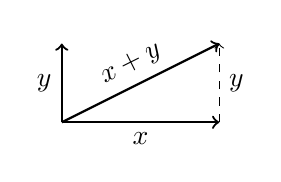
\begin{tikzpicture}
    \draw[thick,->] (0,0) -- (2,0) node[pos=0.5, below] {$x$};
    \draw[thick,->] (0,0) -- (0,1) node[pos=0.5, left] {$y$};
    \draw[thick,->] (0,0) -- (2,1) node[pos=0.5, rotate=26.57, above] {$x+y$};
    \draw[dashed,->] (2,0) -- (2,1) node[pos=0.5, right] {$y$};
\end{tikzpicture}
    \caption{Illustration of the Pythagorean Theorem in the plane}
    \label{fig:sec3-1-ex2}
\end{figure}

\end{exercise}
\begin{proof}
We have
\begin{align*}
    \norm{x+y}^2
    =& \brackets{x+y, x+y}\\
    =& \brackets{x, x+y} + \brackets{y, x+y}\\
    =& \overline{\brackets{x+y, x}} + \overline{\brackets{x+y,y}}\\
    =& \overline{\brackets{x, x} + \brackets{y, x}} + \overline{\brackets{x,y} + \brackets{y,y}}\\
    =& \brackets{x, x} + \brackets{y,y}\\
    =& \norm{x}^2 +\norm{y}^2,
\end{align*}
as required.

Extending the formula to $m$ mutually orthogonal vectors would give us
\begin{align*}
    \norm{x_1+\dots+x_m}^2
    = \norm{x_1}^2 + \dots + \norm{x_m}^2.
\end{align*}
\end{proof}

\begin{exercise}{3}
If $X$ in exercise 2 is real, show that, conversely the given relation implies that $x\perp y$. 
Show that this may not hold if $X$ is complex. Give examples.
\end{exercise}
\begin{proof}
Suppose then that $X$ is real and that $\norm{x+y}^2 = \norm{x}^2 + \norm{y}^2$.
We have
\begin{align*}
    \norm{x}^2 + \norm{y}^2
    =& \norm{x+y}^2\\
    =& \brackets{x+y, x+y}\\
    =& \brackets{x, x+y} + \brackets{y, x+y}\\
    =& \brackets{x+y, x} + \brackets{x+y,y}\\
    =& \brackets{x, x} + \brackets{y, x} 
    + \brackets{x,y} + \brackets{y,y}\\
    =& \norm{x}^2 + \norm{y}^2 + 2\brackets{x,y}.
\end{align*}
Thus $2\brackets{x,y}=0$, so that $x\perp y$.

Now consider $1,i\in\C$. 
We have $\norm{1+i}^2 = 1^2 + 1^2 = \norm{1}^2 + \norm{i}^2$, however, $\brackets{1,i} = -i\brackets{1,1} = -i$, so that they are not orthogonal.
\end{proof}

\begin{exercise}{6}
Let $x\neq 0$ and $y\neq 0$.
\begin{enumerate}
    \item If $x\perp y$, show that $\set{x,y}$ is a linearly independent set.
    \item Extend the result to mutually orthogonal nonzero vectors $x_1,\dots, x_m$.
\end{enumerate}
\end{exercise}
\begin{proof}
\begin{enumerate}
    \item We will prove this by contrapositive.
    Suppose $x$ and $y$ are not linearly independent, so that $x=ay$ for some scalar $a$.
    We then have
    \begin{align*}
        \brackets{x,y}
        = \brackets{ay, y} 
        = a\brackets{y,y} 
        \neq 0,
    \end{align*}
    so that $x$ is not orthogonal to $y$.
    \item There are many ways in which we can extend this idea to many vectors.
    One could be to force $x_i$ to be orthogonal to any linear combination of the rest of the vectors.
\end{enumerate}
\end{proof}

\begin{exercise}{7}
If in an inner product space $\brackets{x,u} = \brackets{x,v}$ for all $x$, show that $u=v$.
\end{exercise}
\begin{proof}
Consider $x=u-v$.
We have
\begin{align*}
    &\brackets{u-v, u} = \brackets{u-v, v} &&\iff\\
    &\brackets{u-v, u} - \brackets{u-v, v} &&\iff\\
    &\overline{\brackets{u, u-v}} - \overline{\brackets{v, u-v}} = 0 &&\iff\\
    &\overline{\brackets{u-v,u-v}} = 0 &&\iff\\
    &\norm{u-v} = 0.
\end{align*}
Norms have the property that $\norm{x} = 0$ if and only if $x=0$, thus $u-v=0$ and $u=v$, as required.
\end{proof}

\begin{exercise}{9}
Prove that
\begin{align*}
    \text{Re}\brackets{x,y} = 1/4[\norm{x+y}^2-\norm{x-y}^2];\quad \text{Im}\brackets{x,y} = 1/4[\norm{x+iy}^2-\norm{x-iy}^2]
\end{align*}
\end{exercise}
\begin{proof}
($\text{Re}\brackets{x,y}$)
We have 
\begin{align*}
    \norm{x+y}^2 = \norm{x}^2 +\norm{y}^2 + \overline{\brackets{y,x}} + \overline{\brackets{x,y}},
\end{align*}
and
\begin{align*}
    \norm{x-y}^2 = 
    \norm{x}^2 +\norm{y}^2 -\overline{\brackets{y,x}} - \overline{\brackets{x,y}}.
\end{align*}
So that
\begin{align*}
    1/4[\norm{x+y}^2 -\norm{x-y}^2]
    =& 1/4[2\overline{\brackets{y,x}} + 2\overline{\brackets{x,y}}]\\
    =& 1/2[2\text{Re}\brackets{x,y}],
\end{align*}
as required.
Where the last equality follows from Axler 4.5, for example.

($\text{Im}\brackets{x,y}$)
We have
\begin{align*}
    \norm{x+iy}^2
    =& \brackets{x+iy, x+iy}\\
    =& \brackets{x,x+iy} + i\brackets{y,x+iy}\\
    =& \overline{\brackets{x+iy,x}} +i\overline{\brackets{x+iy,y}}\\
    =& \overline{\brackets{x,x} + i\brackets{y,x}} + i[\overline{\brackets{x,y} + i\brackets{y,y}}]\\
    =& \norm{x}^2 + \norm{y}^2 - i\overline{\brackets{y,x}} + i\overline{\brackets{x,y}},
\end{align*}
and
\begin{align*}
    \norm{x-iy}^2
    =& \brackets{x-iy, x-iy}\\
    =& \brackets{x,x-iy} - i\brackets{y,x-iy}\\
    =& \overline{\brackets{x-iy,x}} -i\overline{\brackets{x-iy,y}}\\
    =& \overline{\brackets{x,x} - i\brackets{y,x}} - i[\overline{\brackets{x,y} - i\brackets{y,y}}]\\
    =& \norm{x}^2 + \norm{y}^2 + i\overline{\brackets{y,x}} - i\overline{\brackets{x,y}}.
\end{align*}
We use these two together to obtain
\begin{align*}
    1/4[\norm{x+iy}^2-\norm{x-iy}^2]
    =& 1/4[i2\overline{\brackets{x,y}} -i2\overline{\brackets{y,x}}]\\
    =& -i/2[\brackets{x,y}-\overline{\brackets{x,y}}\\
    =& -i/2[2i\text{Im}(x,y)] = \text{Im}\brackets{x,y},
\end{align*}
as required.
\end{proof}

\begin{exercise}{10}
Let $x$ and $y$ denote complex numbers.
Show that $\brackets{x,y} = x\bar{y}$ defines an inner product, which yields the usual metric on the complex plane.
Under what condition do we have orthogonality?
\end{exercise}
\begin{proof}
(IP1)
Suppose $z\in\C$.
We have 
\begin{align*}
    \brackets{(x+y),z}
    = (x+y)\bar{z}
    = x\bar{z} + y\bar{z}
    = \brackets{x,z} + \brackets{y,z}.
\end{align*}

(IP2)
Suppose $a\in\C$.
We have
\begin{align*}
    \brackets{ax,y}
    = ax\bar{y}
    = a\brackets{x,y}.
\end{align*}

(IP3)
We have
\begin{align*}
    \overline{\brackets{x,y}}
    = \overline{x\bar{y}}
    = \bar{x}\overline{\bar{y}}
    = \bar{x}y
    = y\bar{x}
    = \brackets{y,x}.
\end{align*}

(IP4)
We have
\begin{align*}
    \brackets{x,x}
    = x\bar{x}
    = \absoluteValue{x}^2 \geq 0,
\end{align*}
with equality if and only if $x=0$.

(Orthogonality)
Write $x=a+bi$ and $y=c+di$.
We then have
\begin{align*}
    0
    =& \brackets{x,y} && \iff\\
    =& (a+bi)\overline{(c+di)} &&\iff\\
    =& ac - aci + cbi - bdi^2 &&\iff\\
    =& (ac+bd) + (cb-ad)i.
\end{align*}
So orthogonolity holds when $ac=-bd$ and $cb=ad$.
\end{proof}

\begin{exercise}{11}
Let $X$ be the vector space of all ordered pairs of complex numbers.
Can we obtain the norm defined on $X$ by $\norm{x} =\absoluteValue{x_1}+\absoluteValue{x_2}$ from an inner product?
\end{exercise}
\begin{proof}
No, consider $x =(1,1), y=(1,-1) \in\C$.
We have
\begin{align*}
    &\norm{x+y}^2 = \absoluteValue{2}^2\\
    &\norm{x-y}^2 = \absoluteValue{2}^2\\
    &\norm{x}^2 = \sqrt{1^2+1^2}^2\\
    &\norm{y}^2 = \sqrt{1^2+(-1)^2}^2.
\end{align*}
Thus the parallelogram equality
\begin{align*}
    \norm{x+y}^2 + \norm{x-y}^2 = 
    2[\norm{x}^2 + \norm{y}^2]
\end{align*}
does not hold, and thus the norm cannot be obtained by an inner product.
\end{proof}

\begin{exercise}{15}
If $X$ is a finite dimensional vector space and $(e_j)$ is a basis for $X$, show that an inner product on $X$ is completely determined by its values $\gamma_{jk}=\brackets{e_j,e_k}$.
Can we choose such scalars $\gamma_{jk}$ in a completely arbitrary fashion?
\end{exercise}
\begin{proof}
Take any $x,x'\in X$.
We have 
\begin{align*}
    \brackets{x,x'}
    =& \brackets{a_1e_1+\dots+a_ne_n, a_1'e_1+\dots+a_n'e_n}\\
    =& \brackets{a_1e_1,a_1'e_1+\dots+a_n'e_n} + \dots + \brackets{a_ne_n,a_1'e_1+\dots+a_n'e_n}\\
    =& \overline{\brackets{a_1'e_1+\dots+a_n'e_n, a_1e_1}} + \dots + \overline{\brackets{a_1'e_1+\dots+a_n'e_n, a_ne_n}}\\
    =& \overline{\brackets{a_1'e_1, a_1e_1}} + \dots \overline{\brackets{a_n'e_n, a_1e_1}} + \dots + \overline{\brackets{a_1'e_1, a_ne_n}} + \dots +
    \overline{\brackets{a_n'e_n, a_ne_n}}\\
    =& \overline{a_1'\bar{a_1}\brackets{e_1, e_1}} + \dots \overline{a_n'\bar{a_1}\brackets{e_n, e_1}} + \dots + \overline{a_1'\bar{a_n}\brackets{e_1, e_n}} + \dots +
    \overline{a_n'\bar{a_n}\brackets{e_n, e_n}}\\
    =& \overline{a_1'\bar{a_1}\gamma_{1,1}} + \dots \overline{a_n'\bar{a_1}\gamma_{n,1}} + \dots + \overline{a_1'\bar{a_n}\gamma_{1,n}} + \dots +
    \overline{a_n'\bar{a_n}\gamma_{n,n}}.
\end{align*}
so that the value of the inner product is completely determined by $\gamma_{j,k}$.

For $\gamma_{j,k}$ to be valid, we need $\gamma_{j,j}>0$ and $\gamma_{j,k}=\overline{\gamma_{k,j}}$, which implies that the matrix representing the inner product is self-adjoint.
\end{proof}


\section{Fundamental theorems for normed and Banach spaces}
\subsection{Open sets}

No exercises

\section{Further applications: Banach fixed point Theorem}
\subsection{Banach fixed point Theorem}

\begin{exercise}{1}
fill
\end{exercise}
\begin{proof}
fill
\end{proof}

\section{Further applications: approximation theory}
\subsection{Approximation in normed spaces}

\begin{exercise}{1}
fill
\end{exercise}
\begin{proof}
fill
\end{proof}

\section{Spectral theory of linear operators in normed spaces}
\section{Spectral theory in finite dimensional normed spaces}

\begin{exercise}{x}
fill
\end{exercise}
\begin{proof}
fill
\end{proof} 

\begin{exercise}{x}
fill
\end{exercise}
\begin{proof}
fill
\end{proof} 

\begin{exercise}{x}
fill
\end{exercise}
\begin{proof}
fill
\end{proof} 

\begin{exercise}{x}
fill
\end{exercise}
\begin{proof}
fill
\end{proof} 

\begin{exercise}{x}
fill
\end{exercise}
\begin{proof}
fill
\end{proof} 

\begin{exercise}{x}
fill
\end{exercise}
\begin{proof}
fill
\end{proof} 

\begin{exercise}{x}
fill
\end{exercise}
\begin{proof}
fill
\end{proof} 

\begin{exercise}{x}
fill
\end{exercise}
\begin{proof}
fill
\end{proof} 

\begin{exercise}{x}
fill
\end{exercise}
\begin{proof}
fill
\end{proof} 

\begin{exercise}{x}
fill
\end{exercise}
\begin{proof}
fill
\end{proof} 

\begin{exercise}{x}
fill
\end{exercise}
\begin{proof}
fill
\end{proof} 

\begin{exercise}{x}
fill
\end{exercise}
\begin{proof}
fill
\end{proof} 

\begin{exercise}{x}
fill
\end{exercise}
\begin{proof}
fill
\end{proof} 

\begin{exercise}{x}
fill
\end{exercise}
\begin{proof}
fill
\end{proof} 

\begin{exercise}{x}
fill
\end{exercise}
\begin{proof}
fill
\end{proof} 

\begin{exercise}{x}
fill
\end{exercise}
\begin{proof}
fill
\end{proof} 

\begin{exercise}{x}
fill
\end{exercise}
\begin{proof}
fill
\end{proof} 

\begin{exercise}{x}
fill
\end{exercise}
\begin{proof}
fill
\end{proof} 

\begin{exercise}{x}
fill
\end{exercise}
\begin{proof}
fill
\end{proof} 

\section{Compact linear operators on normed spaces and their spectrum}
\subsection{Compact linear operators on normed spaces}

\begin{exercise}{1}
fill
\end{exercise}
\begin{proof}
fill
\end{proof}

\section{Spectral theory of bounded self-adjoint linear operators}
\section{Spectral properties of bounded self-adjoint linear operators}

\begin{exercise}{x}
fill
\end{exercise}
\begin{proof}
fill
\end{proof} 

\begin{exercise}{x}
fill
\end{exercise}
\begin{proof}
fill
\end{proof} 

\begin{exercise}{x}
fill
\end{exercise}
\begin{proof}
fill
\end{proof} 

\begin{exercise}{x}
fill
\end{exercise}
\begin{proof}
fill
\end{proof} 

\begin{exercise}{x}
fill
\end{exercise}
\begin{proof}
fill
\end{proof} 

\begin{exercise}{x}
fill
\end{exercise}
\begin{proof}
fill
\end{proof} 

\begin{exercise}{x}
fill
\end{exercise}
\begin{proof}
fill
\end{proof} 

\begin{exercise}{x}
fill
\end{exercise}
\begin{proof}
fill
\end{proof} 

\begin{exercise}{x}
fill
\end{exercise}
\begin{proof}
fill
\end{proof} 

\begin{exercise}{x}
fill
\end{exercise}
\begin{proof}
fill
\end{proof} 

\begin{exercise}{x}
fill
\end{exercise}
\begin{proof}
fill
\end{proof} 

\begin{exercise}{x}
fill
\end{exercise}
\begin{proof}
fill
\end{proof} 

\begin{exercise}{x}
fill
\end{exercise}
\begin{proof}
fill
\end{proof} 

\begin{exercise}{x}
fill
\end{exercise}
\begin{proof}
fill
\end{proof} 

\begin{exercise}{x}
fill
\end{exercise}
\begin{proof}
fill
\end{proof} 

\begin{exercise}{x}
fill
\end{exercise}
\begin{proof}
fill
\end{proof} 

\begin{exercise}{x}
fill
\end{exercise}
\begin{proof}
fill
\end{proof} 

\begin{exercise}{x}
fill
\end{exercise}
\begin{proof}
fill
\end{proof} 

\begin{exercise}{x}
fill
\end{exercise}
\begin{proof}
fill
\end{proof} 

\section{Unbounded linear operators in Hilbert space}
\section{Unbounded linear operators and their Hilbert-adjoint operators}

\begin{exercise}{x}
fill
\end{exercise}
\begin{proof}
fill
\end{proof} 

\begin{exercise}{x}
fill
\end{exercise}
\begin{proof}
fill
\end{proof} 

\begin{exercise}{x}
fill
\end{exercise}
\begin{proof}
fill
\end{proof} 

\begin{exercise}{x}
fill
\end{exercise}
\begin{proof}
fill
\end{proof} 

\begin{exercise}{x}
fill
\end{exercise}
\begin{proof}
fill
\end{proof} 

\begin{exercise}{x}
fill
\end{exercise}
\begin{proof}
fill
\end{proof} 

\begin{exercise}{x}
fill
\end{exercise}
\begin{proof}
fill
\end{proof} 

\begin{exercise}{x}
fill
\end{exercise}
\begin{proof}
fill
\end{proof} 

\begin{exercise}{x}
fill
\end{exercise}
\begin{proof}
fill
\end{proof} 

\begin{exercise}{x}
fill
\end{exercise}
\begin{proof}
fill
\end{proof} 

\begin{exercise}{x}
fill
\end{exercise}
\begin{proof}
fill
\end{proof} 

\begin{exercise}{x}
fill
\end{exercise}
\begin{proof}
fill
\end{proof} 

\begin{exercise}{x}
fill
\end{exercise}
\begin{proof}
fill
\end{proof} 

\begin{exercise}{x}
fill
\end{exercise}
\begin{proof}
fill
\end{proof} 

\begin{exercise}{x}
fill
\end{exercise}
\begin{proof}
fill
\end{proof} 

\begin{exercise}{x}
fill
\end{exercise}
\begin{proof}
fill
\end{proof} 

\begin{exercise}{x}
fill
\end{exercise}
\begin{proof}
fill
\end{proof} 

\begin{exercise}{x}
fill
\end{exercise}
\begin{proof}
fill
\end{proof} 

\begin{exercise}{x}
fill
\end{exercise}
\begin{proof}
fill
\end{proof} 

\section{Unbounded linear operators in quantum mechanics}
\subsection{Basic ideas. States. Observables, position operator}

\begin{exercise}{1}
fill
\end{exercise}
\begin{proof}
fill
\end{proof}

\end{document}